\glsreset{de}
\glsreset{ea}
\chapter{Der Lösungsansatz}
\label{sec:sol}

	Dieses Kapitel beginnt mit einer Einführung in die Evolutionären Algorithmen und stellt daraus exemplarisch die Differentielle Evolution vor. Zum Schluss dieses Kapitels folgt eine Einbindung der Differentiellen Evolution in den Kontext der Segmentierung.

	\section{\gls{ea}}
	\label{sec:evol}
	
		Hierbei handelt es sich, wie in \cite{ea-intro} beschrieben, um heuristische Verfahren zur Lösung von Problemen, die andernfalls nicht in polynomialer Zeit gelöst werden können. Dabei orientieren sie sich an den Vorgängen der biologischen Evolution. Die Begründung hierfür wird von John H. Holland \cite{j-h-holland} in prägnanter Weise dargelegt: 
	
		\begin{quote}
			\textit{Lebewesen sind vollendete Problemlöser. In der Vielzahl der Aufgaben, die sie bewältigen, übertreffen sie die besten Computerprogramme bei weitem - zur besonderen Frustration der Programmierer, die Monate oder gar Jahre harter geistiger Arbeit für einen Algorithmus aufwenden, während Organismen ihre Fähigkeiten durch den scheinbar ziellosen Mechanismus der Evolution erwerben.}
		\end{quote}
	
		Dieses Zitat bietet eine grobe Vorstellung vom Wesen und der Herkunft von \gls{ea}. In vielen literarischen Werken zu diesem Thema - beispielsweise \cite{ger-kla-kru-intro, eib-smi-ea} - wird festgehalten, dass verschiedene Kategorien von \gls{ea}s existieren. Allerdings ist die zugrunde liegende Idee hinter all diesen Sorten von Algorithmen die selbe und wird von den Autoren in \cite{eib-smi-ea} wie folgt dargelegt:\\
		Gegeben sei eine Gruppe von Individuen, genannt \textit{Population}, die innerhalb einer Umgebung mit begrenzten Ressourcen lebt. Der Kampf um diese löst eine natürliche Selektion aus und führt so zu einer höheren Fitness der Population - ein Vorgang, der sehr gut unter dem Stichwort \textit{Survival of the Fittest} bekannt ist. Nach diesem Vorbild aus der Natur nehme man
		\begin{itemize}
			\item ein zu lösendes Problem (stellvertretend für die Umgebung), abgebildet durch eine (Fitness-)Funktion, die maximiert oder minimiert werden soll, sowie
			\item eine Menge an Lösungskandidaten (im Folgenden als Individuen bezeichnet), bestehend aus einem Set von Funktionsparameterlisten.
		\end{itemize}
		Auf diese Individuen wird sodann die Fitnessfunktion angewendet und mit dem Ergebnis in abstrakter Weise jeweils die Fitness der einzelnen Individuen gemessen. Dabei erfolgt die Bewertung abhängig davon, ob minimiert oder maximiert werden soll. Im folgenden Schritt erzeugen verschiedene Variationsoperatoren wie Mutation und/oder Rekombination aus der Ursprungspopulation eine neue Population, für die wiederum die Fitnessfunktion ausgewertet wird. Auf der Basis der jeweiligen Fitnesswerte werden die korrespondierenden Individuen beider Populationen verglichen und davon dasjenige mit der höheren Fitness in die Population der nächsten Generation übernommen.
	
		Die oben genannten Schritte werden so lange iteriert, bis entweder eine geeignete Lösung gefunden wurde oder eine (vorher definierte) maximale Anzahl an Iterationen erreicht ist. Abbildung \ref{fig:ea-flowchart}. veranschaulicht die Funktionsweise von \gls{ea}s nochmals in Form eines einfachen Flussdiagramms.
	
		\begin{figure}[h]
			\centering
			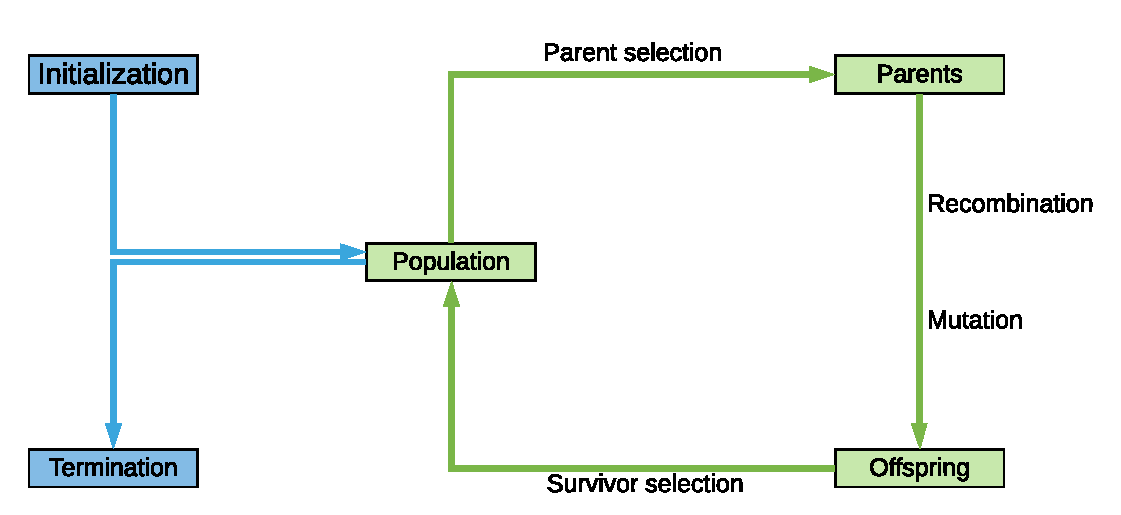
\includegraphics[width=\linewidth]{ea_flowchart}
			\caption[Genereller Ablauf von \gls{ea}s]{Genereller Ablauf von \gls{ea}s (Nachbildung der Graphik aus \cite[Seite 27]{eib-smi-ea})}
			\label{fig:ea-flowchart}
		\end{figure}
	
		Nachstehend wird in Abschnitt \ref{sec:de} die Methode der 
		\textit{Differentiellen Evolution} als Beispiel vorgestellt und in den 
		weiteren Kontext der vorliegenden Arbeit eingebettet.
	
		\glsreset{de}

	\section{\gls{de}}
	\label{sec:de}

		Die Autoren in \cite{storn-price-de} entwickelten diese Methode mit Hinblick auf die im Anschluss gelisteten Anforderungen an ein in der Praxis anwendbares Optimierungsverfahren:
		\begin{enumerate}
			\item Es soll mit nicht-differenzierbaren und nicht-linearen 
			Funktionen, die unter Umständen mehrere (lokale) Maxima/Minima 
			aufweisen, umgehen können.
			\item Falls eine sehr rechenintensive Funktion auftritt, soll das 
			Verfahren parallelisierbar sein. Es soll also möglich sein, die 
			Berechnungen auf mehrere Prozessorkerne auszulagern.
			\item Weiterhin soll die Methode leicht zu benutzen sein. Im 
			gegebenen Kontext bedeutet dies zum Beispiel, dass sie wenige 
			Kontrollparameter besitzt, die einfach bestimmbar sind.
			\item Außerdem soll sie sich mit steigender Iterationszahl immer 
			näher dem \textbf{globalen} Minimum/Maximum annähern.
		\end{enumerate}
		Zwar ist \gls{de} laut \cite{storn-price-de} darauf ausgerichtet, die 
		oben genannten Bedingungen zu erfüllen, den Wahrheitsgehalt dieser 
		Aussage zu prüfen soll jedoch nicht Aufgabe der hier vorliegenden 
		Arbeit sein. Hier liegt der Fokus primär auf der Anwendung des 
		Verfahrens mit der Annahme, die vorangestellte Aussage sei wahr.\\
		
		Der nachstehende Pseudocode beschreibt die substanzielle Idee hinter \gls{de} in etwas vereinfachter Form \cite{storn-price-de}:
		
		\begin{algorithm*}[H]
			\SetAlgoLined
			...\\
			\While{convergence criterion not yet met}{
				//---$x_{i}$ defines a vector of the current vector population-------\\
				//---$y_{i}$ defines a vector of the new vector population-----------\\
				for ($i=0$; $i<N_{p}$; i++) \{\\
				\begin{tabbing}
					Links \= Mitte \= Rechts \kill
					\>$r_{1} = rand(N_{p});$ //select a random index from $1, 2, ..., N_{p}$\\
					\>$r_{2} = rand(N_{p});$ //select a random index from $1, 2, ..., N_{p}$\\
					\>$r_{3} = rand(N_{p});$ //select a random index from $1, 2, ..., N_{p}$\\
					\>\textbf{$u_{i} = x_{r_{3}} + F * (x_{r_{1}} - x_{r_{2}})$};\\
					\>\textbf{if} $f(u_{i}) \leq f(x_{i})$  \textbf{then} \{\\
						\>\>$y_{i} = u_{i};$\\
					\>\} \textbf{else} \{\\
						\>\>$y_{i} = x_{i};$\\
					\>\}\\
					\}
				\end{tabbing}
			}
			...
		\end{algorithm*}
	
		mit $N_{p}$ für die Größe der Population stehend.\\
		Mit der Zeit haben sich unterschiedliche Varianten von \gls{de} herausgebildet. Die gängige Notation hierfür folgt dem Schema \textit{\gls{de}/x/y/z}, wobei sich die Bedeutung der Variablen x, y und z im Verlauf der nachfolgenden detaillierten Beschreibung der einzelnen Operationen in \gls{de} an geeigneter Stelle erschließen werden \cite{storn-price-de, storn-price-de-book}. 
		%\vfill
		
		\subsection{Initialisierung}
		\label{sec:de-init}
		
			Zunächst muss die initiale Population ($G = 0$) erzeugt werden - 
			meist durch Befüllen der Parametervektoren $x_{i, 0}$ mit 
			Zufallszahlen. Im Bezug auf diese Zufallszahlen sowie alle 
			kommenden wird eine Gleichverteilung angenommen. In manchen Fällen 
			ist eine vorläufige Lösung $x_{nom, 0}$ verfügbar - dann kann die 
			Population durch Addieren zufälliger Abweichungen zu $x_{nom, 0}$ 
			generiert werden. Die nachfolgenden Operationen werden so lange 
			iteriert, bis die vorher festgelegte Anzahl an Generationen $G$ 
			erreicht ist. \color{red} [Formel!!] \color{black}
			
		\subsection{Mutation}
		\label{sec:de-mutation}
		
			Für alle $x_{i, g}$ werden Mutantenvektoren $v_{i, g+1}$ gebildet. 
			Hierfür gibt es unterschiedliche Rechenvorschriften, abhängig 
			davon, die \gls{de}-Variante gewählt ist. Hierzu werden im 
			Folgenden einige häufig vorkommende Beispiele dargelegt (die 
			jeweils letzten Parameter werden in Paragraph 
			\ref{sec:de-crossover} eingehender beleuchtet, da sie hier keine 
			Auswirkungen zeigen):
			\color{red} [Formel Formatierung anpassen] \color{black}
			
			{\Large
				\setlength{\abovedisplayskip}{0pt}
				\setlength{\abovedisplayshortskip}{0pt}
				\begin{flalign}
					\label{eq:mutation1}
					&\textrm{\gls{de}/\textcolor{blue}{rand}/\textcolor{green}{1}/bin:}&v_{i,
					 g+1} = \color{blue}x_{r_{1}, g} \color{black}+ 
					F \cdot \color{green}(x_{r_{1}, g} - x_{r_{2}, g})&&
				\end{flalign}
			}%
			{\Large
				\setlength{\abovedisplayskip}{0pt}
				\setlength{\abovedisplayshortskip}{0pt}
				\begin{flalign}
					\label{eq:mutation2}
					&\textrm{\gls{de}/\textcolor{blue}{best}/\textcolor{green}{1}/bin:}&v_{i,
					 g+1} &= \color{blue}x_{best, g} \color{black}+ 
					F \cdot \color{green}(x_{r_{1}, g} - x_{r_{2}, g})&&
				\end{flalign}
			}%
			{\Large
				\setlength{\abovedisplayskip}{0pt}
				\setlength{\abovedisplayshortskip}{0pt}
				\begin{flalign}
					\label{eq:mutation3}
					&\textrm{\gls{de}/\textcolor{blue}{best}/\textcolor{green}{2}/exp:}&v_{i,
					 g+1} &= \color{blue}x_{best, g} \color{black}+ 
					F \cdot \color{green}((x_{r_{1}, g} + x_{r_{2}, g}) - 
					(x_{r_{3}, g} + 
					x_{r_{4}, g}))&&
				\end{flalign}
			}%
			$\forall i \in [1,2, ..., N_{p}]$ mit $r_{1}$, $r_{2}$, $r_{3}$ und 
			$r_{4}$ als zufällige, 
			voneinander und auch von $i$ unterschiedliche Indices und 
			\textit{best} als Index desjenigen Vektors der Generation g, 
			der bei Auswertung mit der Fitnessfunktion den 
			niedrigsten/höchsten Wert innerhalb der Population liefert.
			
		\subsection{Crossover}
		\label{sec:de-crossover}
		
			Das Ergebnis der Crossover-Operation ist eine neue Population, die 
			beim Selektionsvorgang in Paragraph \ref{sec:de-selection} mit der 
			Ursprungspopulation konkurriert, mit den Vektoren $u_{i, g+1}$ und 
			ihren Parametern $u_{j, i, g+1}$ mit $j = 1, 2, ... , D$. Deren 
			Ermittlung kann ebenfalls je nach Abwandlung von \gls{de} 
			unterschiedliche Formen annehmen:
			\color{red} [Formel!!] \color{black}
			
			
		\subsection{Selektion}
		\label{sec:de-selection}
		\color{red} [Formel!!] \color{black}
			
			
	\section{Die Testumgebung}
	\label{sec:testsetting}
